\chapter{Results and Discussion}\label{sec:results}


% ==================
%\iffalse
% =-------------------

\section{Poisson and Diffusion Solvers}

Setting up a composite multi-scale simulation where multiple equations are coupled requires a profound understanding of the model components. 
Thus, it can help to first simulate isolated models. We provide simple examples with our software, such as Laplace and Diffusion problems, as prototypes for elliptic and parabolic partial differential equations. The examples with analytic solutions are also used to validate the basic finite element solvers.

In this section, we showcase three of these simple problems. First, we consider the 1D Poisson problem $u''(x) = f$ on $\Omega=[0,1]$ with Dirichlet boundary conditions $u(0)=0$ and $u(1)=1$ and right hand side $f(x)=6\,x$. The analytic solution is $y(x)=x^3$. \Cref{fig:poisson} shows the analytic solution and the results of the finite element computation with linear and quadratic ansatz functions for two elements. Both linear and quadratic finite element solutions cannot exactly represent the cubic function, however, yield the best possible approximation. 
The first bidomain equation given in \cref{eq:bidomain1} is a 3D version of this Poisson problem and is needed in the multi-domain model to simulate EMG signals on the muscle surface.

The second example is a 2D Laplace problem $c(x)\,\Delta u(x) = 0$. The solution is given in \cref{fig:laplace_composite_1} and can be interpreted as a static electric potential field. 
The mesh uses quadratic Lagrange ansatz functions and is composed of two joined rectangular parts, each given by a structured mesh. The conductivity is set to $c=1$ in the left part and to $c=2$ in the right part. Dirichlet boundary conditions prescribe the electric potential at the five upper points in the right mesh to $u = -1$ and at the center of the right mesh to $u=1$. In addition, Neumann boundary conditions $\partial u / \partial \bfn = -1$ corresponding to an outward electric current are set on the left boundary of the left mesh with the normal vector $\bfn$ pointing to the left. \Cref{fig:laplace_composite_1} visualizes the degree of freedom values of the right hand side contribution of the Neumann boundary conditions by the arrows. 
A 3D Laplace problem is also part of the multi-scale model and describes volume conduction in the adipose tissue domain as formulated in \cref{eq:body}.

% poisson - laplace
\begin{figure}
  \centering%
  \begin{subfigure}[t]{0.38\textwidth}%
    \centering%
    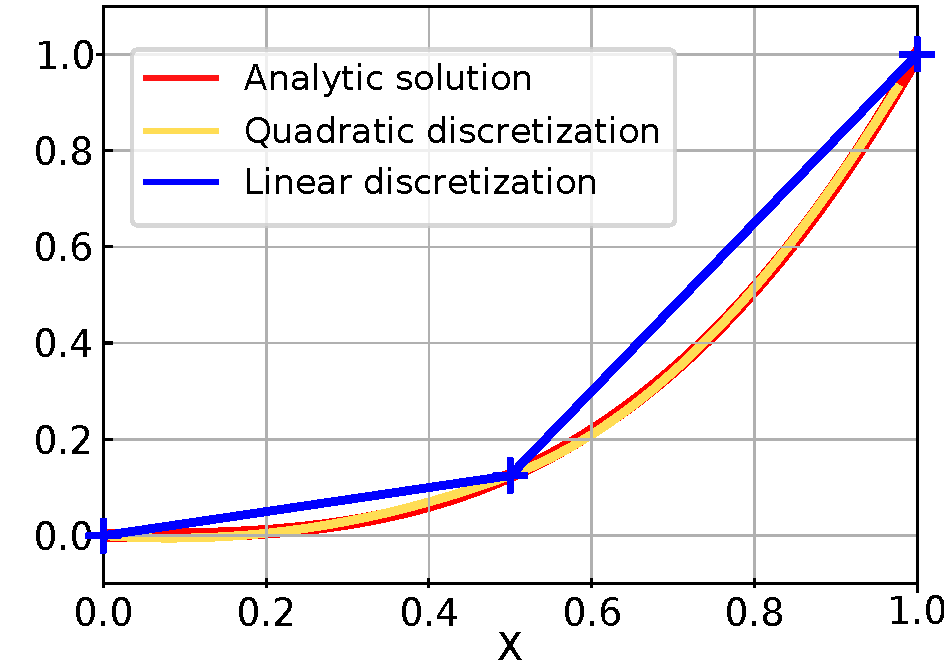
\includegraphics[width=\textwidth]{images/results/basic/analytic.pdf}%
    \caption{Solution of a Poisson problem for linear and quadratic ansatz functions.}%
    \label{fig:poisson}%
  \end{subfigure}\quad
  \begin{subfigure}[t]{0.58\textwidth}%
    \centering%
    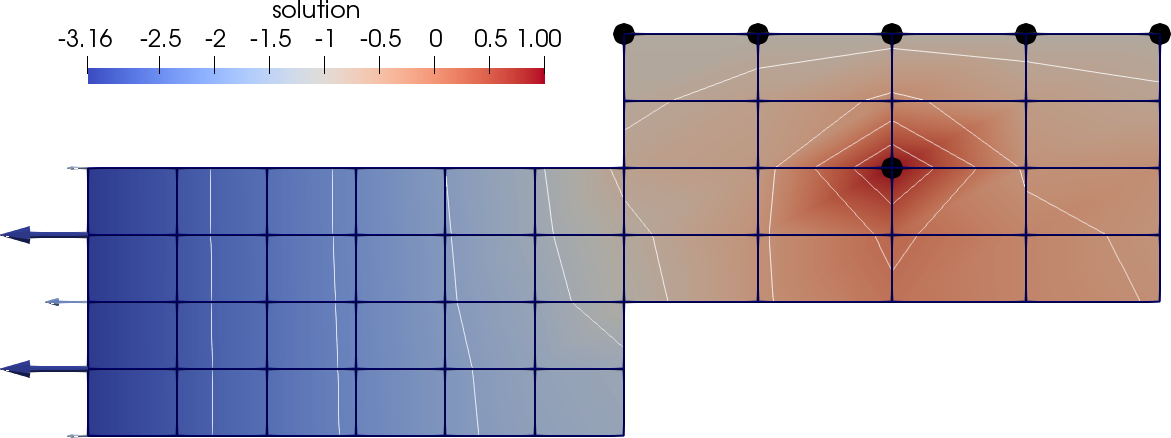
\includegraphics[width=\textwidth]{images/results/basic/laplace_composite_1.png}%
    \caption{Finite element mesh and solution of a 2D electric conduction problem .}%
    \label{fig:laplace_composite_1}%
  \end{subfigure}
  \caption{Exemplary problems that can be solved with OpenDiHu and are part of the multi-scale problem.}%
  \label{fig:diffusion}%
\end{figure}%

The third presented example solves the 2D diffusion equation $\partial u/\partial t - \div(\bfsigma\,\grad u) = 0$ with homogeneous Neumann boundary conditions. The equation can be interpreted as a transient electric conduction problem. As shown in \cref{fig:diffusion1}, the initial charge distribution is $u=1$ in a rectangle in the inner of the domain and $u=0$ everywhere else. The anisotropic conduction tensor $\bfsigma$ is constant in the domain and set to %
\begin{align*}
  \bfsigma = \frac15\,\mat{1 & 1\\
              1 & 6}.
\end{align*}
A linear mesh with $40\times 40$ elements is used. \Cref{fig:diffusion2} shows the solution at time $t=5$, where the initially discontinuous charge distribution has smoothed out and has expanded mainly in $y$ direction, which is the preferential direction of electric conduction in this example. A 3D version of this equation is part of the multidomain model and given by \cref{eq:multidomain1}.

% diffusion
\begin{figure}
  \centering%
  \begin{subfigure}[t]{0.4\textwidth}%
    \centering%
    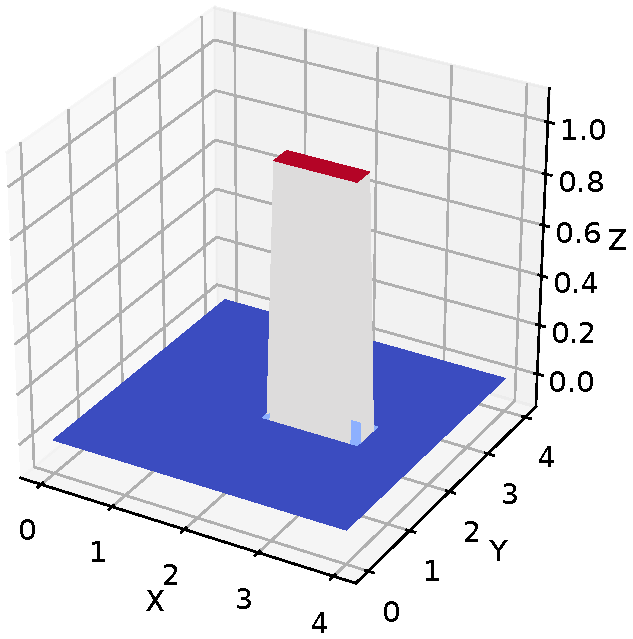
\includegraphics[width=\textwidth]{images/results/basic/diffusion1.pdf}%
    \caption{Initial charge distribution, $t=0$.}%
    \label{fig:diffusion1}%
  \end{subfigure}\quad
  \begin{subfigure}[t]{0.4\textwidth}%
    \centering%
    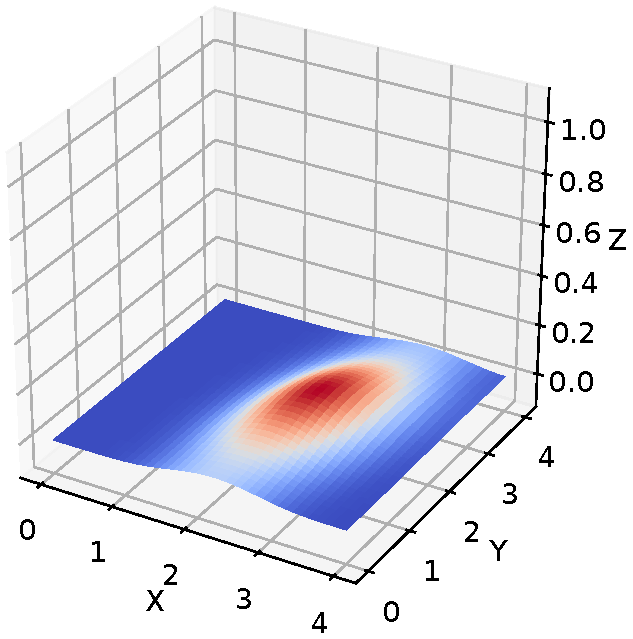
\includegraphics[width=\textwidth]{images/results/basic/diffusion2.pdf}%
    \caption{Solution at $t=5$.}%
    \label{fig:diffusion2}%
  \end{subfigure}
  \caption{A 2D electric conduction problem as a demonstrator for the solution of transient problems in OpenDiHu.}%
  \label{fig:diffusion}%
\end{figure}%


\begin{reproduce_no_break}
  The three presented simulations can be executed and visualized as follows:
  \begin{lstlisting}[columns=fullflexible,breaklines=true,postbreak=\mbox{\textcolor{gray}{$\hookrightarrow$}\space},language=python]
    cd $\$$OPENDIHU_HOME/examples/poisson/poisson1d_2/build_release
    ./linear ../settings_1d.py && plot out/*.py
    ./quadratic ../settings_1d.py && plot out/*.py
    ./hermite ../settings_1d.py && plot out/*.py

    cd $\$$OPENDIHU_HOME/examples/laplace/laplace_composite/build_release/
    ./laplace_composite_2d ../settings_2d_2.py && paraview paraview_state.pvsm

    cd $\$$OPENDIHU_HOME/examples/diffusion/anisotropic_diffusion/build_release
    ./anisotropic_diffusion2d ../settings2d.py && plot out/*.py
  \end{lstlisting}
\end{reproduce_no_break}

%-----
\section{Solid Mechanics Solver}

Next, we demonstrate the solid mechanics solvers, which can be used to compute muscle contraction. In this section, we focus on the passive material behavior.
As described in \cref{sec:material_linear_model,sec:material_modeling}, the mechanics equations can be computed in linearized or in nonlinear form within OpenDiHu.
In the following, \cref{sec:comparison_linear_nonlinear} applies both model approaches in a simulation of an externally stretched muscle and compares the results. Then, \cref{sec:validation_nonlinear} validates the implementation of the nonlinear hyperelasticity solver in OpenDiHu. Finally, \cref{sec:simulation_hyperelastic_tendon} showcases, using the simulation of a tendon, how more complex material models can be computed.

%-----
\subsection{Comparison of Linear and Nonlinear Mechanics Models}\label{sec:comparison_linear_nonlinear}

We demonstrate the use of linear and nonlinear mechanics models in a simulation of an externally stretched biceps muscle. The muscle belly is fixed at its lower end and an upwards pulling force acts on the upper end, effectively stretching the muscle tissue in vertical direction.

We solve two scenarios with the same geometry and boundary conditions but different material models. The first scenario uses the linearized mechanics model given in \cref{sec:material_linear_model}. We use material parameters obtained from porcine in vitro indentor tests in literature \cite{schock1982vivo} and set the bulk modulus to $K=\SI{39}{\kilo\pascal}$ and the shear modulus to $\mu=\SI{48}{\kilo\pascal}$.

The second scenario uses the incompressible transversely isotropic hyperelastic muscle material based on the Mooney-Rivlin description without active stress, which is defined in \cref{sec:material_nonlinear_model}. The material parameters are set to the values given \cite{Heidlauf2016}.

\Cref{fig:lin_nonlin_muscle_mechanics} shows the geometric setup of the model. We discretize the biceps geometry by a quadratic 3D mesh with 252  elements and a total of $13 \times 13 \times 15 = 2535$ nodes.
The linearized material model uses this mesh to construct the stiffness matrix and solve the linear system.
For the nonlinear model, an additional coarser linear mesh is constructed and linear-quadratic Taylor-Hood elements are used for the discretization. 

A total force of $(F_x,F_y,F_z) = (0,\SI{-0.4}{\newton},\SI{-3}{\newton})$ is applied, which points in negative $z$-direction, i.e., upwards in \cref{fig:lin_nonlin_muscle_mechanics}, and slightly in negative $y$-direction, i.e, to the left in \cref{fig:lin_nonlin_muscle_mechanics}.
Instead of a single force vector acting on a point, the equivalent constant surface load is applied on the whole top face of the muscle geometry.

We consider a static problem where no timestepping is required. In the linear model, the resulting displacements are obtained by a GMRES solver that solves the linear system of equations \cref{eq:linearized_helper4} corresponding  to the finite element formulation.
The nonlinear model uses increasing load steps, which are adaptively refined in case the solver diverges at one load step. The scheme solves a system of nonlinear equations for every load step, and the contained linear system is solved by a direct solver.

% linear and nonlinear mechanics solvers
\begin{figure}
  \centering%
  \hfill
  \begin{subfigure}[t]{0.4\textwidth}%
    \centering%
    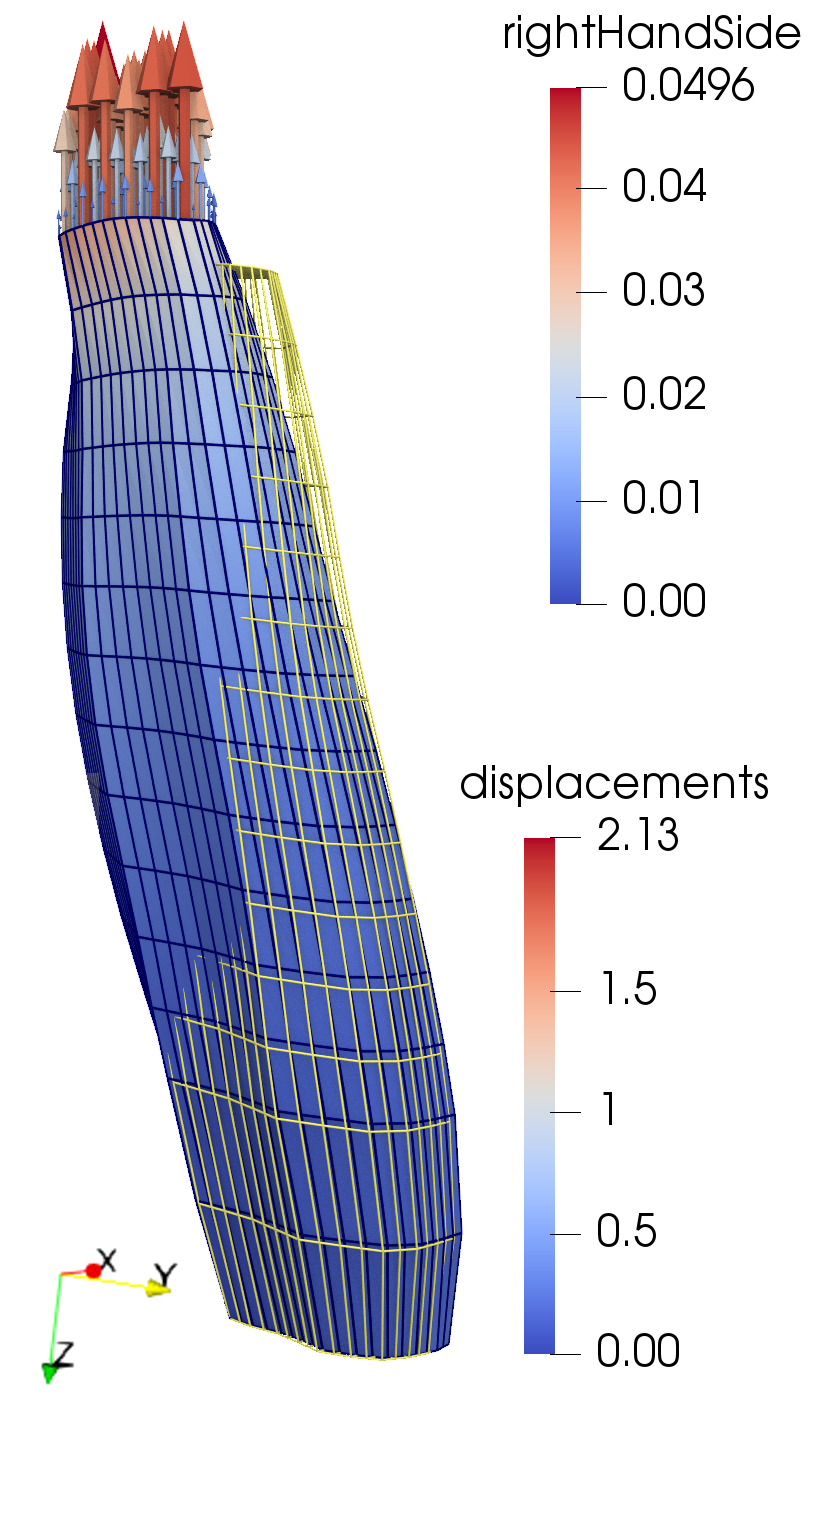
\includegraphics[height=12cm]{images/results/basic/lin_nonlin_muscle_mechanics_b.png}%
    \caption{Solution of the linear model.}%
    \label{fig:lin_nonlin_muscle_mechanics_b}%
  \end{subfigure}\hfill
  \begin{subfigure}[t]{0.4\textwidth}%
    \centering%
    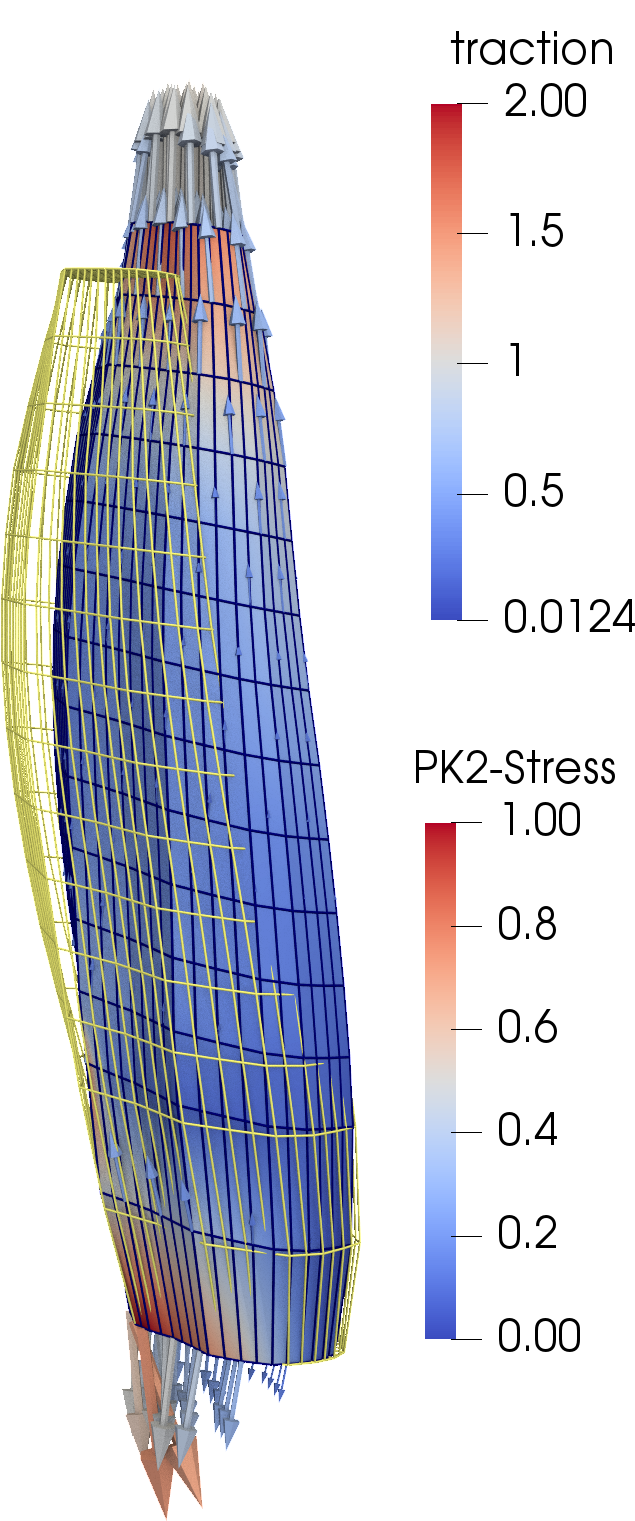
\includegraphics[height=12cm]{images/results/basic/lin_nonlin_muscle_mechanics_a.png}%
    \caption{Solution of the nonlinear model.}%
    \label{fig:lin_nonlin_muscle_mechanics_a}%
  \end{subfigure}
  \hfill
  \caption{Comparison of linear and nonlinear mechanics models. A biceps muscle is stretched by an applied force.}%
  \label{fig:lin_nonlin_muscle_mechanics}%
\end{figure}%

The results of the linear and nonlinear models are shown in \cref{fig:lin_nonlin_muscle_mechanics_b,fig:lin_nonlin_muscle_mechanics_a}. 
In both images, the identical reference configuration is given by the yellow wireframe and the deformed muscle is given by the solid body with colored mesh. 
The deformed body in the linear model in \cref{fig:lin_nonlin_muscle_mechanics_b} is colored according to the resulting vector of unknowns, which contains the displacements.  Arrows on the upper end of the geometry indicate the negative right hand side of the linear system as formulated in \cref{eq:linearized_mechanics_rhs}. The arrows correspond to the applied Neumann boundary conditions in the weak form of the finite element formulation and point in the direction of the applied surface load.

In the visualization of the nonlinear model in \cref{fig:lin_nonlin_muscle_mechanics_a}, the deformed muscle body is colored according to the second Piola-Kirchhoff (PK2) stress. It can be seen that the stress is highest at the bottom bearing and at the top end where the muscle cross section is smaller. The arrows visualize the traction forces $\bft$ on virtual horizontal cuts. As a result, the arrows that can be seen on top of the muscle geometry correspond to the applied external force an the arrows at the bottom indicate the forces on the bearing.

A comparison of the two obtained results from the linear and nonlinear models shows a qualitatively different outcome. With the linear model, the muscle bends to the left, whereas with the nonlinear model, it bends to the right. This effect is a result of the different material behavior. The linear model is isotropic and the deformation follows the direction of the applied force, which points to the upper left. The nonlinear model has an anisotropy and is stiffer in fiber direction. As a consequence, the muscle deforms less in longitudinal direction and therefore moves to the right.
Thus, the material models influence the bending direction in this scenario.

In a second example, we compare the muscle stretches that results from different external forces acting in $z$-direction.  We use the same scenario as before and increase the applied force from 0 to \SI{15}{\newton}. We measure the displacement of one node in the top face of the muscle, for both the linear model and the nonlinear model. While the stress-strain relations  in 1D extension tests  can be derived analytically for linear and nonlinear models, our examples considers a real 3D setting where this relation is influenced by the geometry, e.g., by non-parallel fiber directions, as the force is not applied exactly in fiber direction.

\Cref{fig:linear_nonlinear_displacements} shows the resulting muscle extensions for different applied external forces for the linear and nonlinear models.
It can be seen that the stretch of the muscle increases nonlinearly for the transversely isotropic hyperelastic model, in contrast to the linear progression of the linear model.
The slopes of the two curves are qualitatively different, which is a result of the chosen material parameters from different experimental origins. It would be possible to scale the linear model to better match the nonlinear model behavior by simply reducing the value of the bulk modulus accordingly.

% study of displacements, linear  nonlinnear
\begin{figure}
  \centering%
  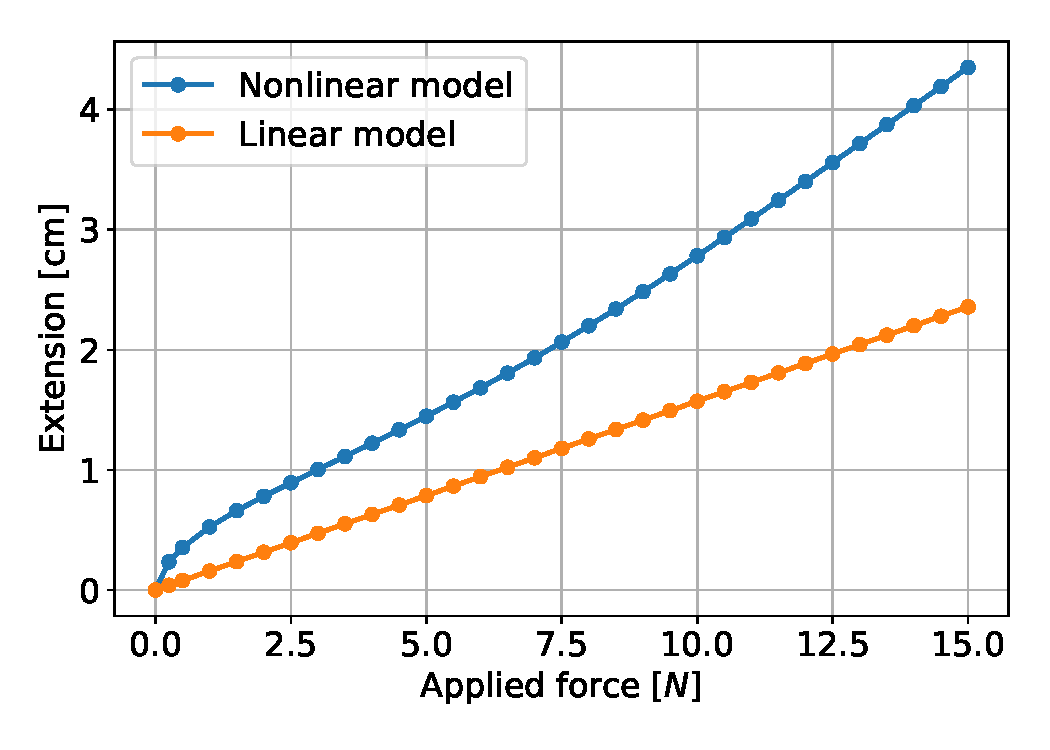
\includegraphics[width=0.7\textwidth]{images/results/basic/linear_nonlinear_displacements.pdf}%
  \caption{Quantitative comparison of the relation between applied force and extension of the muscle for a linear and a nonlinear solid mechanics model.}%
  \label{fig:linear_nonlinear_displacements}%
\end{figure}

The two presented studies show that a linear isotropic material model can give significantly different results than a more accurate nonlinear transversly isotropic model. Therefore, simulations of muscle contraction that target high accuracy should use the according nonlinear models. Nevertheless, both approaches are implemented and can be used with OpenDiHu.

\begin{reproduce_no_break}
  The two simulations for \cref{fig:lin_nonlin_muscle_mechanics} can be run as follows:
  \begin{lstlisting}[columns=fullflexible,breaklines=true,postbreak=\mbox{\textcolor{gray}{$\hookrightarrow$}\space}]
    cd $\$$OPENDIHU_HOME/examples/solid_mechanics/linear_elasticity/muscle/build_release
    ./linear_elasticity ../settings_linear_elasticity.py
    cd $\$$OPENDIHU_HOME/examples/solid_mechanics/mooney_rivlin_transiso/build_release
    ./3d_hyperelasticity ../settings_3d_muscle.py --njacobi=1
  \end{lstlisting}
  The study in \cref{fig:linear_nonlinear_displacements} can be run and plotted using the scripts in the repository at \href{https://github.com/dihu-stuttgart/performance}{github.com/dihu-stuttgart/performance}
  in the directory \code{opendihu/}\\\code{23_linear_nonlinear_mechanics}.
\end{reproduce_no_break}

%-----
\subsection{Validation of the Nonlinear Solid Mechanics Solver}\label{sec:validation_nonlinear}

Next, we perform tests to validate our implementation of the nonlinear hyperelasticity solvers.
We simulate the same scenario with our software and the nonlinear finite element analysis tool \emph{FEBio} \cite{Maas2012}.
FEBio is developed at the University of Utah and the Columbia University in the USA. FEBio contains solid mechanics solvers that can be run from the command line or a graphical user interface model. An extensive model library contains material models also from the domain of biomechanics. The mechanics solver uses the PARDISO linear solver \cite{pardiso2020}, which exploits shared memory parallelism.

An adapter in OpenDiHu exists, which can output the required configuration file for FEBio, run the solver, and parse the computed solution from the text files that are output by FEBio. Thus, we can conduct our validation studies fully in OpenDiHu by using similar Python settings files and the same meshes for the computation in OpenDiHu and the reference solution computed by FEBio.

Apart from the present study, the FEBio adapter in OpenDiHu can also be used to solve quasi-static coupled problems with the electrophysiology part solved in OpenDiHu and the mechanics part solved in FEBio. However, test have shown that the interfacing method of generating configuration files and parsing result files in every timestep leads to higher runtimes than directly using the mechanics solver of OpenDiHu.

In our validation studies, we consider a cube of unit dimensions that is discretized by $8\times 8 \times 8$ quadratic elements and 4913 degrees of freedom. \Cref{fig:tensile_shear_test_img} shows the discretized cube in yellow color. Its orientation is given by the coordinate frame in the lower left of \cref{fig:tensile_test_img}. 
The following Dirichlet boundary conditions are prescribed: All points of the lower face are fixed at $z=0$. The points of the two edges ($y=0 \wedge z=0$) and ($x=0 \wedge z=0$) are additionally fixed in $y$ and $x$ directions, respectively. The corner at $x=y=z=0$ is fixed completely. Thus, the cube can freely deform in its bottom plane, but not move nor rotate. 

% visualization of the scenarios
\begin{figure}
  \centering%
  \hfill
  \begin{subfigure}[t]{0.45\textwidth}%
    \centering%
    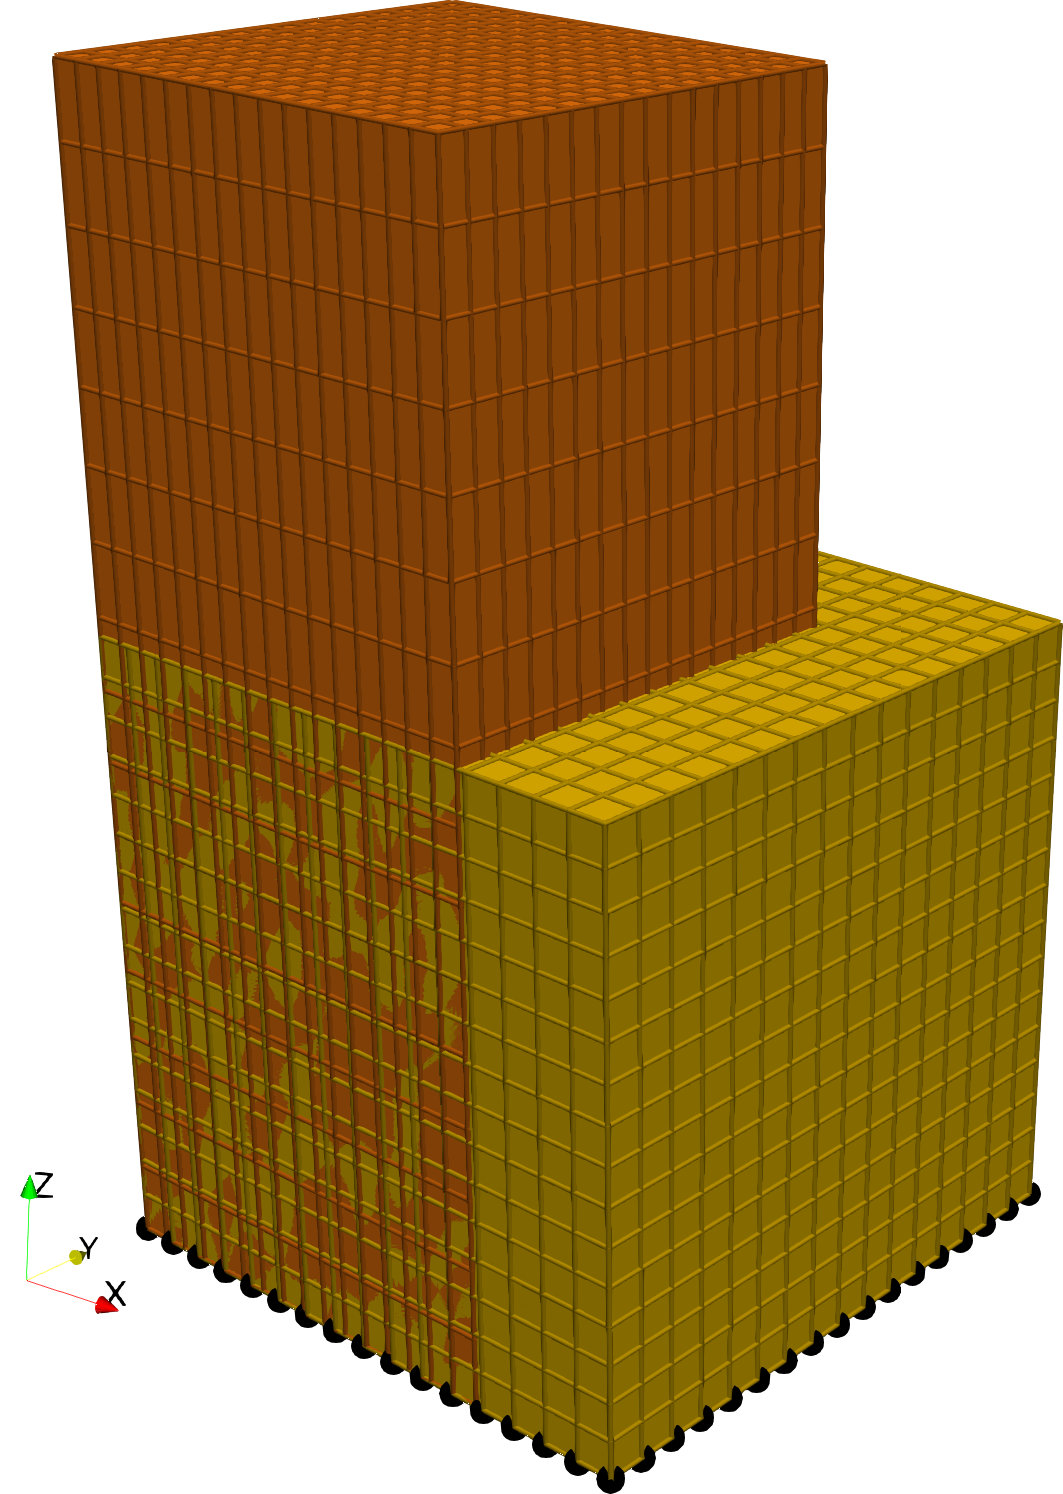
\includegraphics[height=8cm]{images/results/basic/tensile_test_img.png}%
    \caption{Tensile test scenario used in the first validation experiment.}%
    \label{fig:tensile_test_img}%
  \end{subfigure}\hfill
  \begin{subfigure}[t]{0.45\textwidth}%
    \centering%
    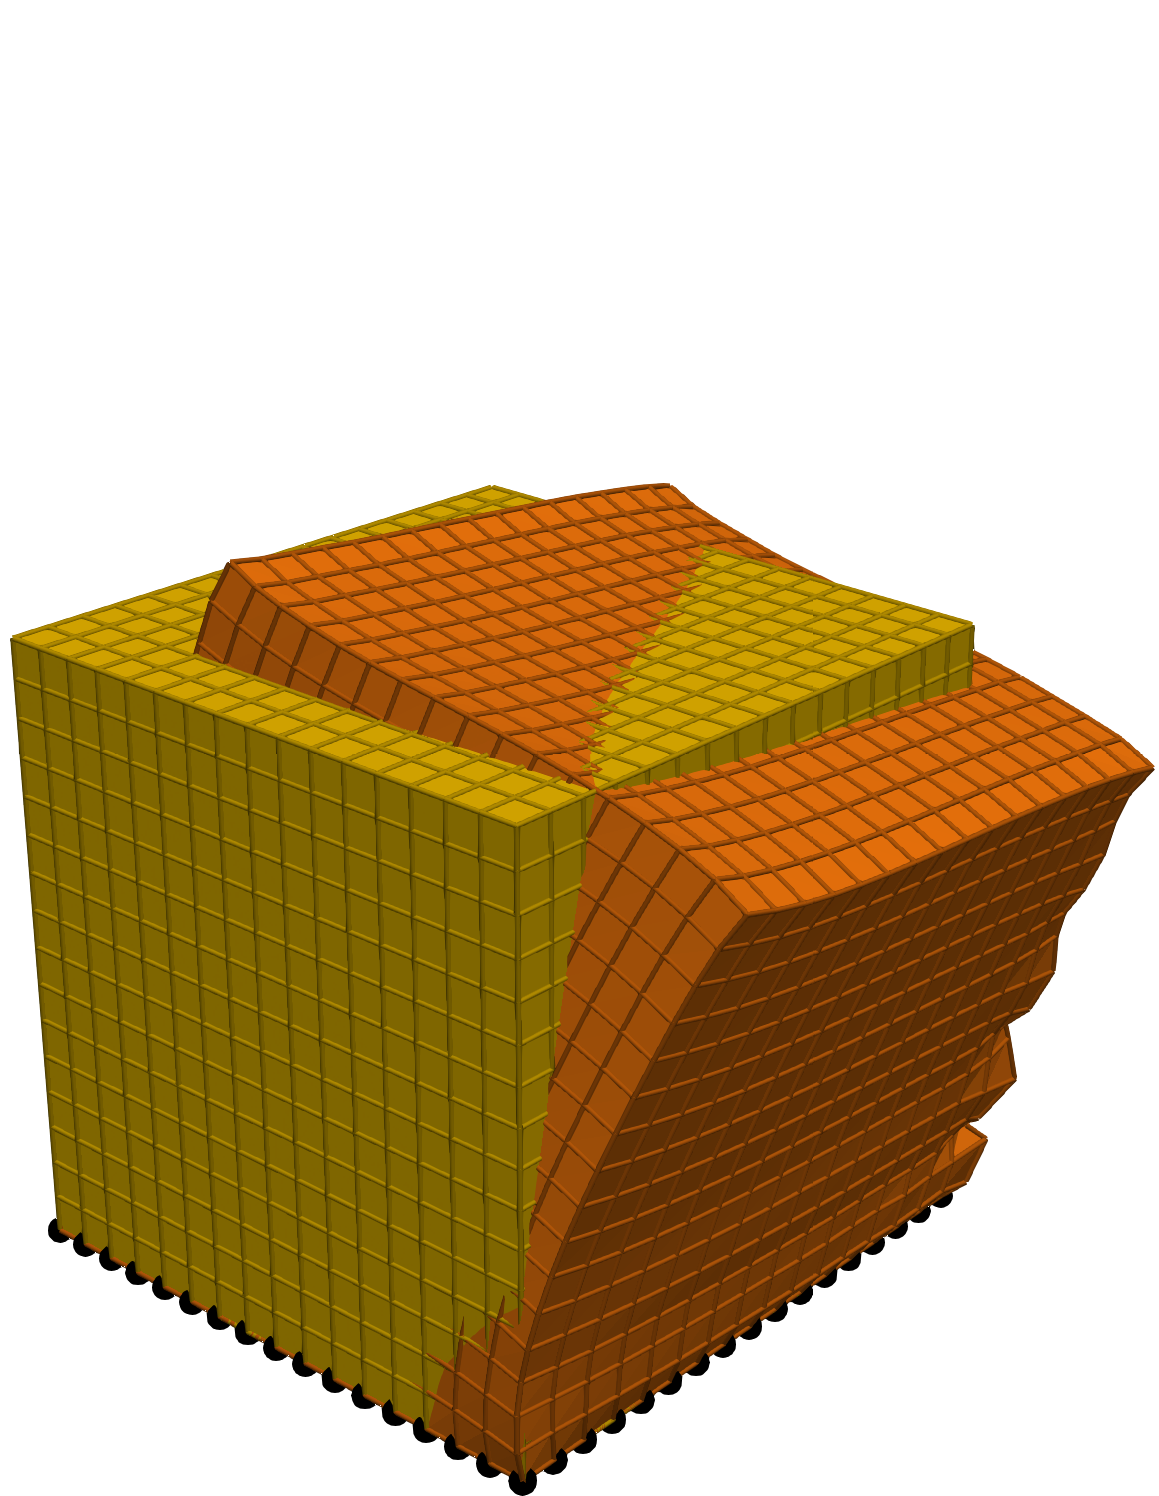
\includegraphics[height=8cm]{images/results/basic/shear_test_img.png}%
    \caption{Shear test scenario used in the second validation experiment.}%
    \label{fig:shear_test_img}%
  \end{subfigure}
  \hfill
  \caption{Scenarios used for validation of the solid mechanics solver. The reference and current configurations are given by the yellow and orange meshes, respectively.}%
  \label{fig:tensile_shear_test_img}%
\end{figure}%

The first study is a tensile test, where a uniform surface load pointing in positive $z$ direction is applied on the top face of the cube. We increase the force from 1 to \SI{50}{\newton}. For the largest force, the cube deforms as shown by the orange geometry in \cref{fig:tensile_shear_test_img}. Note that the volume is preserved due to the incompressibility constraint in the material model.

We use an incompressible and isotropic Mooney-Rivlin material with parameters $c_1=c_2=1$. The material can be simulated in three different forms in OpenDiHu. In the following, we list all model formulations in OpenDiHu and the reference formulation in FEBio:
%
\begin{subequations}\label{eq:validation_1}
  \begin{align}
      \Psi_\text{iso}(\bar{I}_1,\bar{I}_2) &= c_1\,(\bar{I}_1 - 3) + c_2\,(\bar{I}_2 - 3), \quad J=1, \label{eq:validation_incompressible}\\[4mm]
      \Psi(I_1,I_2,I_3) &= c_1\,(I_1 - 3) + c_2\,(I_2 - 3) + \kappa\,(\sqrt{I_3} - 1)^2 - d\,\log(\sqrt{I_3}),\label{eq:validation_nearly_incompressible_1} \\
       d &= 2\,(c_1 + 2\,c_2) \label{eq:validation_nearly_incompressible}, \\[4mm]
      \Psi_\text{iso}(\bar{I}_1,\bar{I}_2) &= c_1\,(\bar{I}_1 - 3) + c_2\,(\bar{I}_2 - 3),\label{eq:validation_nearly_incompressible_decoupled_1} \\ 
      \Psi_\text{vol}(J) &= \kappa\,G(J) \quad\text{with }  G(J) = \dfrac14\big(J^2 - 1 - 2\,\log(J)\big) \label{eq:validation_nearly_incompressible_decoupled} \\[4mm]
      \Psi_\text{iso}(\bar{I}_1,\bar{I}_2) &= c_1\,(\bar{I}_1 - 3) + c_2\,(\bar{I}_2 - 3),\label{eq:validation_nearly_incompressible_decoupled_febio_1} \\ 
      \Psi_\text{vol}(J) &= \kappa\,G(J) \quad\text{with } G(J) = \dfrac12\big(\log(J)\big)^2 \label{eq:validation_nearly_incompressible_decoupled_febio}.
  \end{align}
\end{subequations}
%
The first form given in \cref{eq:validation_incompressible} is the \say{fully incompressible}, mixed $u$-$p$ formulation, which ensures incompressiblity using the Lagrange multipliers. The second formulation in \cref{eq:validation_nearly_incompressible_1,eq:validation_nearly_incompressible} is the \say{nearly incompressible} formulation in terms of the invariants $I_1$ to $I_3$. The third model given in \cref{eq:validation_nearly_incompressible_decoupled_1,eq:validation_nearly_incompressible_decoupled} is the nearly incompressible formulation given in decoupled form, in terms of the reduced invariants $\bar{I}_1$ and $\bar{I}_2$.
The last shown formulation in \cref{eq:validation_nearly_incompressible_decoupled_febio_1,eq:validation_nearly_incompressible_decoupled_febio} is the one used in FEBio and also describes a nearly incompressible material in decoupled form, but with a different penalty function $G(J)$.  
For the three nearly incompressible descriptions in \cref{eq:validation_nearly_incompressible_1,eq:validation_nearly_incompressible_decoupled_1,eq:validation_nearly_incompressible_decoupled_febio_1}, we set the incompressiblity parameter to $\kappa=\num{1e3}$.

We compare the resulting normal stress value $S_{33}$ in $z$-direction of the second Piola-Kirchhoff stress tensor $\bfS$ for all formulations listed in \cref{eq:validation_1}. For the tensile test, this stress value is constant throughout the domain. \Cref{fig:validation_tensile_test} shows the computed stresses over the computed strain values.
It can be seen that the three formulations in OpenDiHu yield approximately the same results as the reference solution given by FEBio over the whole range of applied forces.

% results tensile test
\begin{figure}
  \centering%
  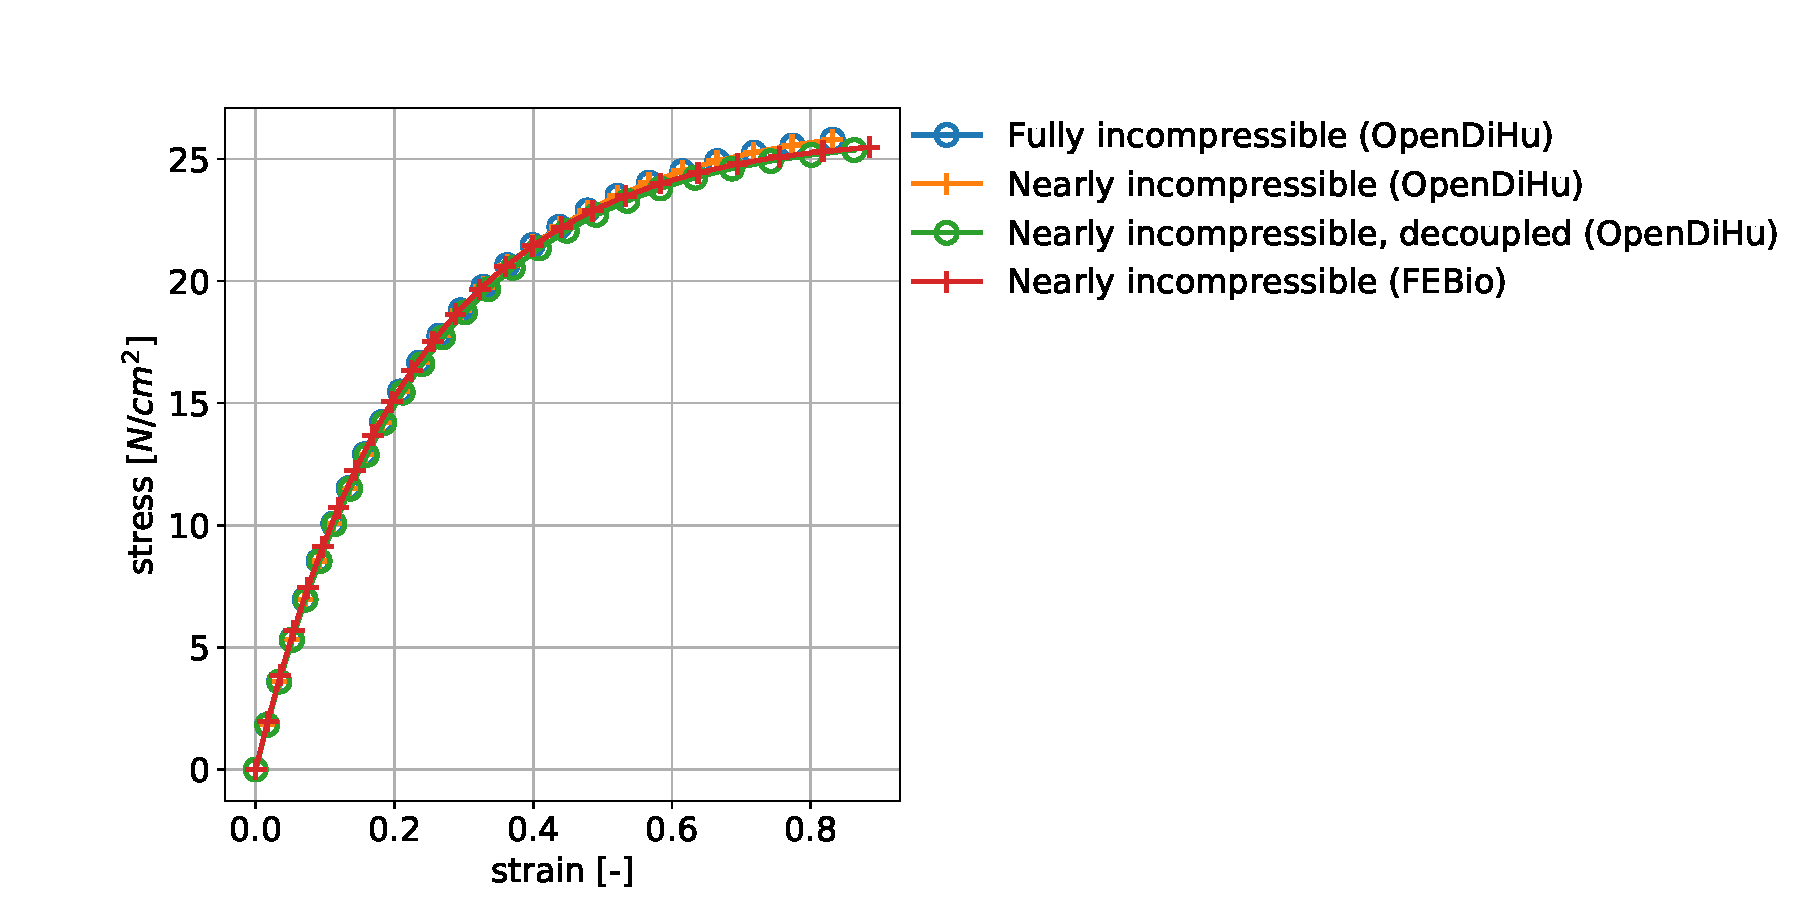
\includegraphics[width=\textwidth]{images/results/basic/validation_tensile_test.pdf}%
  \caption{Results of the tensile test validation experiment. The stress-strain curve for three different formulations in OpenDiHu and the computation in FEBio match.}%
  \label{fig:validation_tensile_test}%
\end{figure}

As the previous tensile test only validates stress and strain in one direction, we additionally conduct a numeric shear experiment. A shear force $\bfF=(0.1\alpha, 0.05\alpha, 0)^\top$ is applied on the top face of the cube and $\alpha$ is again varied between 1 and $\SI{50}{\newton}$. \Cref{fig:shear_test_img} shows the deformed configuration for the highest force by the orange colored body.

% results shear test
\begin{figure}
  \centering%
  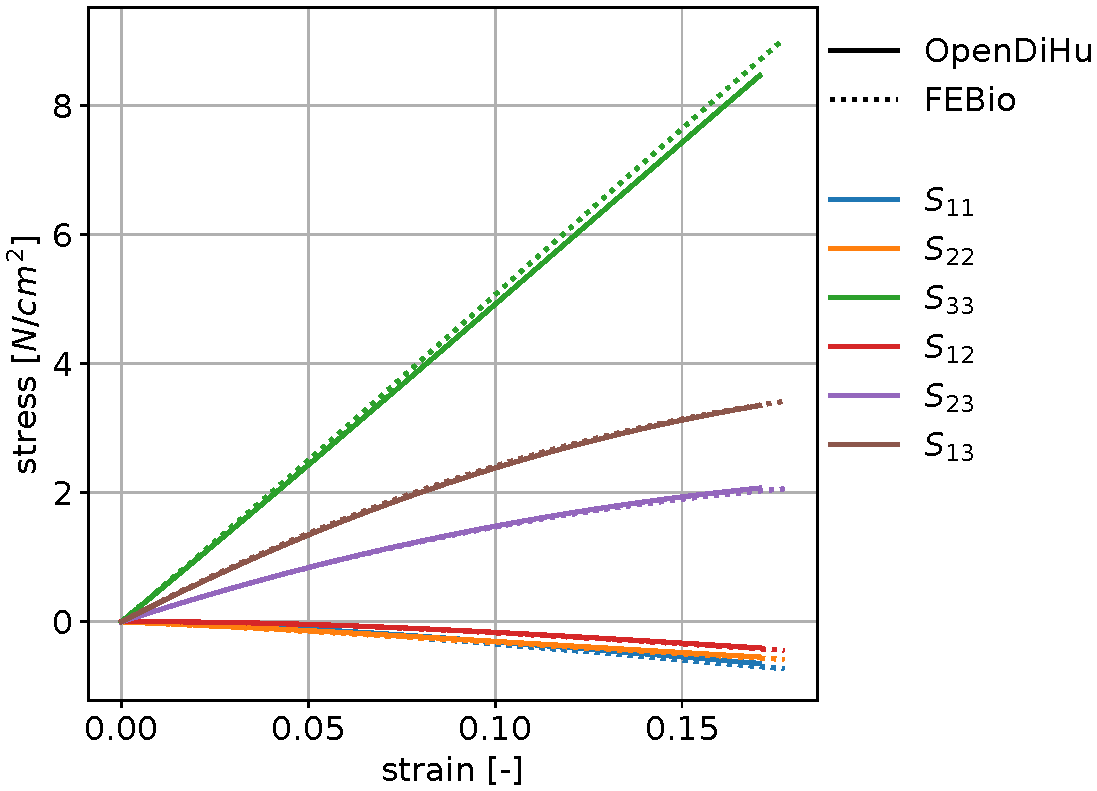
\includegraphics[width=0.6\textwidth]{images/results/basic/validation_shear_test.pdf}%
  \caption{Results of the shear test validation experiment. The values of the second Piola Kirchhoff tensor computed by OpenDiHu (solid lines) and FEBio (dotted lines) closely match.}%
  \label{fig:validation_shear_test}%
\end{figure}

In this second study, we consider one point in the interior of the domain, which is 3 elements below the top face of the mesh. We compare all six distinct entries of the symmetric second Piola-Kirchhoff tensor $\bfS$ between the fully incompressible model in OpenDiHu and the nearly incompressible model in FEBio. 

\Cref{fig:validation_shear_test} shows the computed values in a stress-strain diagram. The solutions of OpenDiHu and FEBio are given by solid and dotted lines, respectively. It can be seen that the curves agree, which validates the implementation in OpenDiHu.

\begin{reproduce_no_break}
  The tensile test validation experiment can be reproduced by the following commands:
  \begin{lstlisting}[columns=fullflexible,breaklines=true,postbreak=\mbox{\textcolor{gray}{$\hookrightarrow$}\space}]
    cd $\$$OPENDIHU_HOME/examples/solid_mechanics/tensile_test/build_release
    ../run_force.sh
    cd $\$$OPENDIHU_HOME/examples/solid_mechanics/tensile_test
    ./plot_validation.py
  \end{lstlisting}
  The shear test can be executed analogously by replacing \code{tensile_test} by \code{shear_test} in the given paths.
\end{reproduce_no_break}

%-----
\subsection{Simulation of a Hyperelastic Tendon Material}\label{sec:simulation_hyperelastic_tendon}

Next, we demonstrate the use of a more complex constitutive material model, which represents tendon tissue. The material is formulated in \cite{Carniel2017}. The model describes microstructural interactions between collagen fibers and their matrix. It consists of a transversely isotropic model that describes the high stiffness in fiber direction and a coupled model for the compressive response. The model is formulated in terms of a logarithmic strain measure.

%from the paper: The high stiffness of tendons under tensile tests is handled by a transversely isotropic model while the coupled compressive response is modeled by means of a Fung-type potential in terms of Seth-Hill’s generalized strain tensors. In present study the logarithm strain measure is used instead of the usually employed Green-Lagrange strain

\Cref{fig:tendon_material_simulation} shows the geometries of the tendons of the biceps brachii and the results of the simulations. The lower tendon in \cref{fig:dynamic_mooney_rivlin_6} is fixed at its left end and a constant surface traction of \SI{1}{\newton} in total pulls to the right. The image shows the initial configuration by the wireframe mesh and the current configuration after $t=\SI{10}{\ms}$, colored according to the resulting velocity.
Similarly, the upper tendons in \cref{fig:dynamic_mooney_rivlin_7} are fixed at the right ends and stretched to the left resulting from the applied force at the left end.

\begin{figure}
  \centering%
  \begin{subfigure}[t]{\textwidth}%
    \centering%
    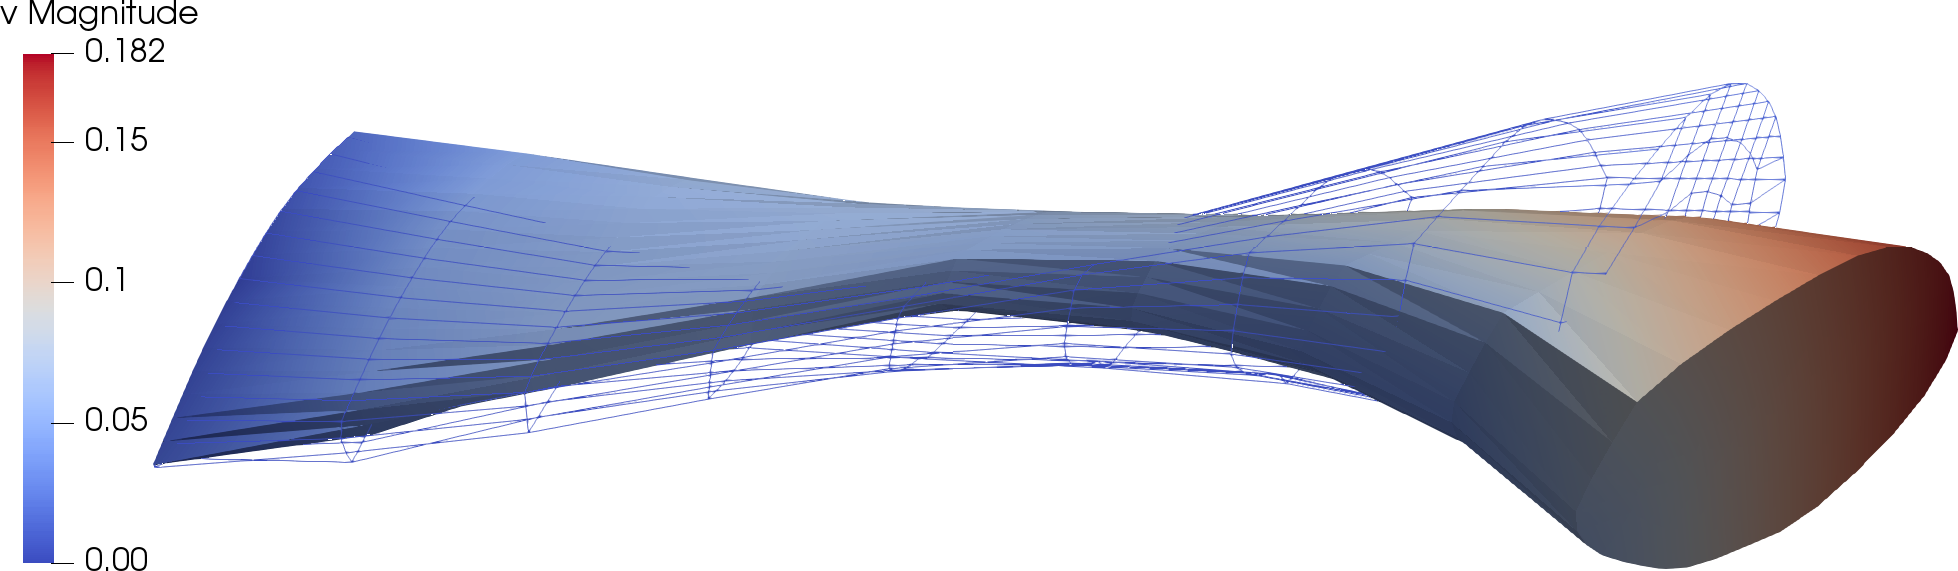
\includegraphics[width=0.9\textwidth]{images/results/basic/dynamic_mooney_rivlin_6.png}%
    \caption{Dynamic simulation of the lower tendon. The attachment to the ulna bone is at the left end. The free right end bends due to the applied surface traction.}%
    \label{fig:dynamic_mooney_rivlin_6}%
  \end{subfigure}\\[4mm]
  \begin{subfigure}[t]{\textwidth}%
    \centering%
    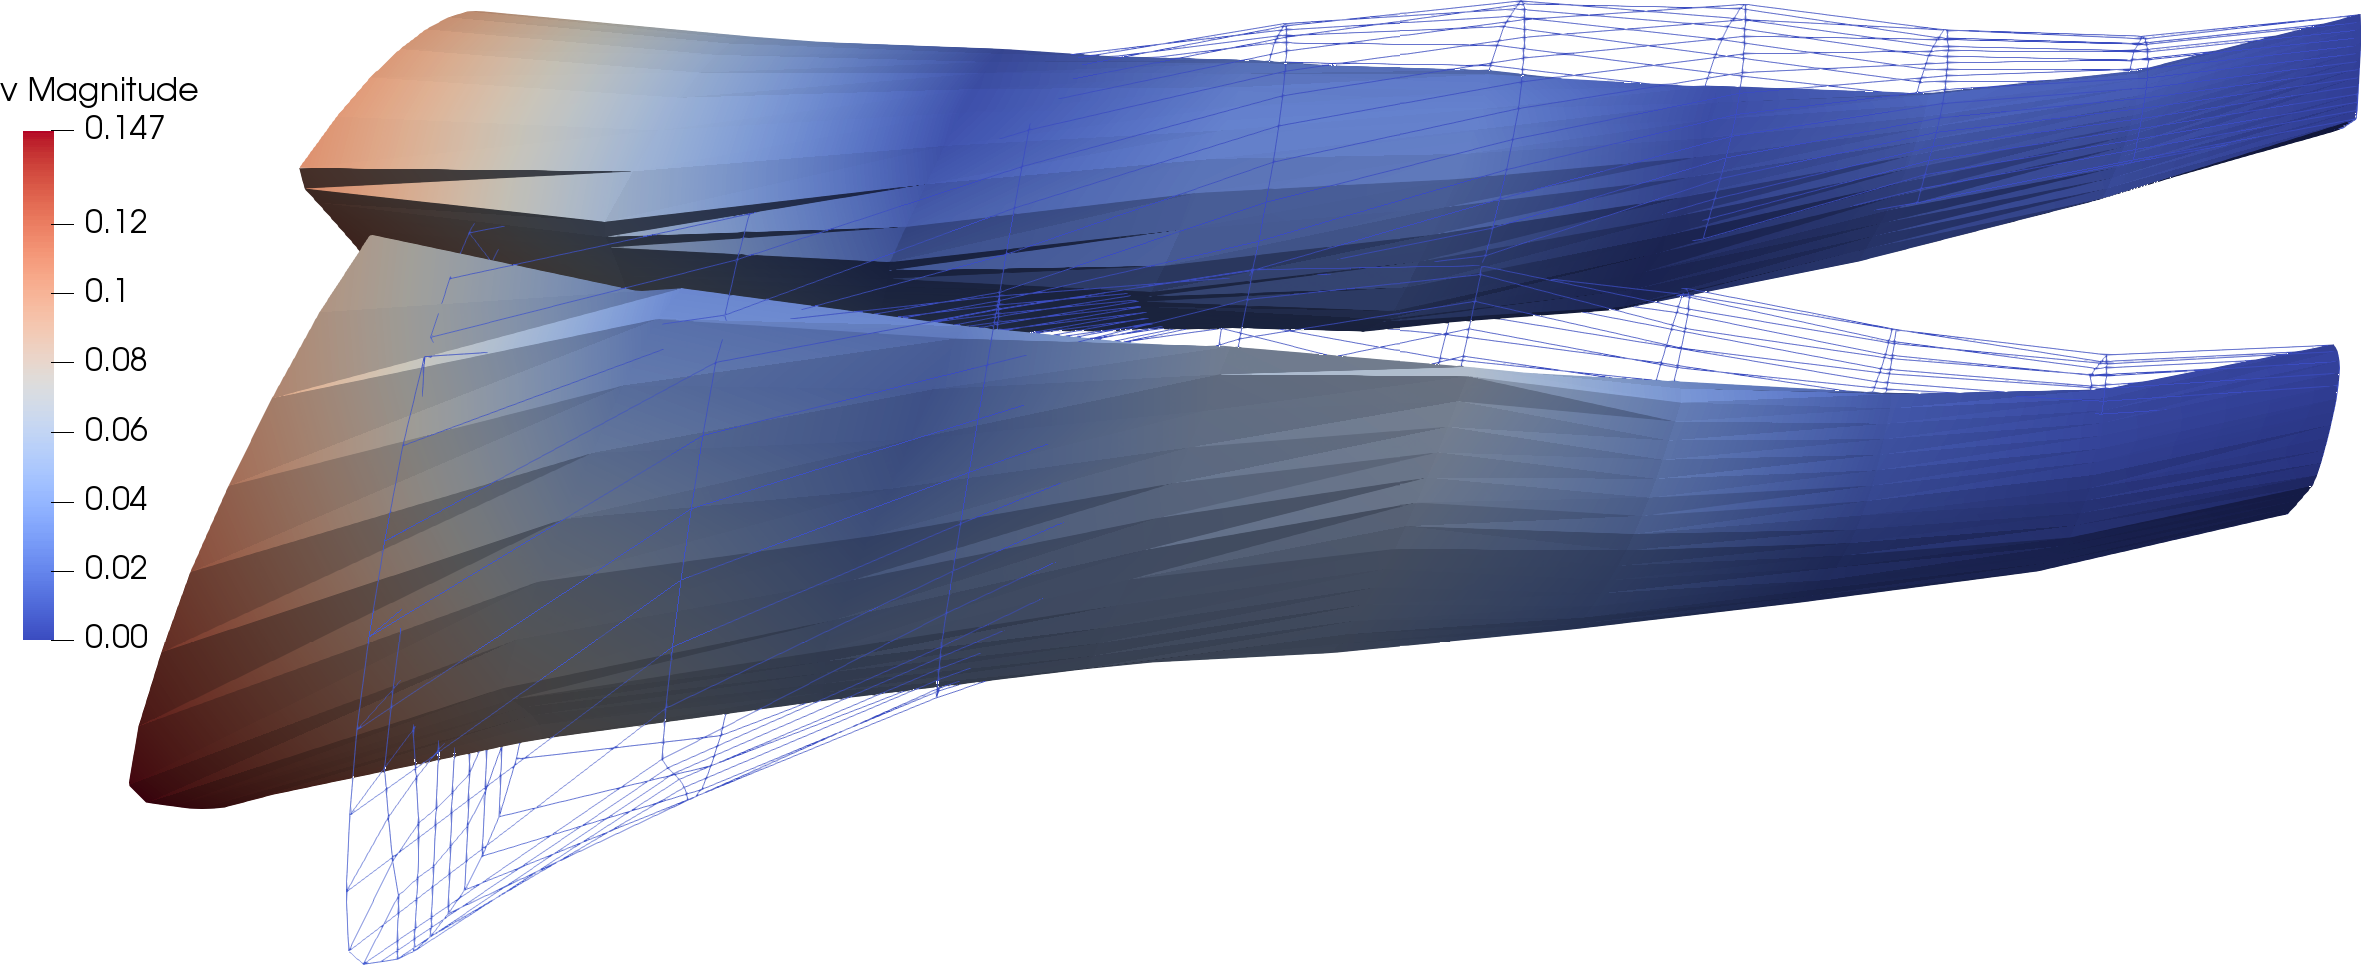
\includegraphics[width=0.9\textwidth]{images/results/basic/dynamic_mooney_rivlin_7.png}%
    \caption{Simulation of the two upper tendons of the two biceps heads.}%
    \label{fig:dynamic_mooney_rivlin_7}%
  \end{subfigure}
  \caption{Simulation of tendons as a showcase of dynamic simulations with complex material models. The color coding indicates the velocity.}%
  \label{fig:tendon_material_simulation}%
\end{figure}%

In summary, this section demonstrated the capabilities of the solid mechanics solvers in OpenDiHu. \Cref{sec:comparison_linear_nonlinear,sec:simulation_hyperelastic_tendon} simulated extension of the biceps muscle and tendons due to external forces. The comparison of results from a linear and a nonlinear model showed that a linear isotropic material cannot always accurately predict the behavior of muscle tissue and, thus, a nonlinear model is required. The validation experiments in \cref{sec:validation_nonlinear} showed that OpenDiHu correctly computes deformation and stresses of incompressible materials.

The solid mechanics solvers can also be coupled to solvers of electrophysiology to simulate muscle contraction resulting from the spatially heterogenous activation and considering the neuronal stimulation dynamics. Such simulations are described later in this work.

% ------------
%\fi
% f===========


